%Version 3.1 December 2024
% See section 11 of the User Manual for version history
%
%%%%%%%%%%%%%%%%%%%%%%%%%%%%%%%%%%%%%%%%%%%%%%%%%%%%%%%%%%%%%%%%%%%%%%
%%                                                                 %%
%% Please do not use \input{...} to include other tex files.       %%
%% Submit your LaTeX manuscript as one .tex document.              %%
%%                                                                 %%
%% All additional figures and files should be attached             %%
%% separately and not embedded in the \TeX\ document itself.       %%
%%                                                                 %%
%%%%%%%%%%%%%%%%%%%%%%%%%%%%%%%%%%%%%%%%%%%%%%%%%%%%%%%%%%%%%%%%%%%%%

%%\documentclass[referee,sn-basic]{sn-jnl}% referee option is meant for double line spacing

%%=======================================================%%
%% to print line numbers in the margin use lineno option %%
%%=======================================================%%

\documentclass[lineno,referee,pdflatex,sn-basic]{sn-jnl}% Basic Springer Nature Reference Style/Chemistry Reference Style

%%%% Standard Packages
%%<additional latex packages if required can be included here>

\usepackage{graphicx}%
\usepackage{multirow}%
\usepackage{amsmath,amssymb,amsfonts}%
\usepackage{amsthm}%
\usepackage{mathrsfs}%
\usepackage[title]{appendix}%
\usepackage{xcolor}%
\usepackage{textcomp}%
\usepackage{manyfoot}%
\usepackage{booktabs}%
\usepackage{algorithm}%
\usepackage{algorithmicx}%
\usepackage{algpseudocode}%
\usepackage{listings}%
%%%%

%%%%%=============================================================================%%%%
%%%%  Remarks: This template is provided to aid authors with the preparation
%%%%  of original research articles intended for submission to journals published 
%%%%  by Springer Nature. The guidance has been prepared in partnership with 
%%%%  production teams to conform to Springer Nature technical requirements. 
%%%%  Editorial and presentation requirements differ among journal portfolios and 
%%%%  research disciplines. You may find sections in this template are irrelevant 
%%%%  to your work and are empowered to omit any such section if allowed by the 
%%%%  journal you intend to submit to. The submission guidelines and policies 
%%%%  of the journal take precedence. A detailed User Manual is available in the 
%%%%  template package for technical guidance.
%%%%%=============================================================================%%%%



\begin{document}

\title[Article Title]{Haemocytes of \textit{Crassostrea virginica} as a dual-purpose source of ultra-long DNA for genome scaffolding and environmental DNA surveillance}

%%=============================================================%%
%% GivenName	-> \fnm{Joergen W.}
%% Particle	-> \spfx{van der} -> surname prefix
%% FamilyName	-> \sur{Ploeg}
%% Suffix	-> \sfx{IV}
%% \author*[1,2]{\fnm{Joergen W.} \spfx{van der} \sur{Ploeg} 
%%  \sfx{IV}}\email{iauthor@gmail.com}
%%=============================================================%%

\author[1]{\fnm{Alyssa} \sur{Strickland}}

\author[2]{\fnm{Kshitij} \sur{Amar}}

\author[1]{\fnm{Bo-Young} \sur{Lee}}

\author[1]{\fnm{Caylin} \sur{Grove}}

\author[2]{\fnm{Miten} \sur{Jain}}

\author*[1]{\fnm{Bonnie L.} \sur{Brown}} \email{bonnie.brown@unh.edu}

\affil*[1]{\orgdiv{Department of Biological Sciences}, \orgname{University of New Hampshire}, \orgaddress{\city{Durham}, \postcode{03874}, \state{NH}, \country{USA}}}

\affil[2]{\orgdiv{Department of Bioengineering}, \orgname{Northeastern University}, \orgaddress{\city{Boston}, \postcode{02115}, \state{MA}, \country{USA}}}

%%==================================%%
%% Sample for unstructured abstract %%
%%==================================%%

\abstract{Sequencing and assembling ultra-long DNA (ULDNA) scaffolds can extend utility of the existing eastern oyster \textit{Crassostrea virginica}, reference genome. In an attempt to create a long-read oyster reference, methodology to successfully isolate ULDNA from eastern oysters was optimized to sequester ultralong oyster DNA from mucopolysaccharides while avoiding excessive shearing. Analysis using a PromethION\texttrademark{} flow cell yielded read lengths (average N50 = 16.5kb, longest read 508kb) that were comparable to what was expected. After quality filtering ($Q \geq 9$), the number of reads $393 \times 10^{3}$ were mapped to 91.4\% of the reference genome (649Mbp, N50=14kb). However, the sequencing coverage was not sufficiently deep to accomplish de novo assembly. Of all ULDNA reads, 94.6\% were successfully mapped to \textit{C. virginica}. Most of the unmapped reads (5.4\% of all reads) were classified to bacteria (56\%) and human (33\%), revealing, respectively, an unexpected oyster pathogen and signaling sewage contamination in the vicinity of oyster harvest.}

\maketitle

\section{Introduction}
Eastern oysters, \textit{Crassostrea virginica}, are both environmentally and economically important in the estuaries where they reside. Eastern oysters provide reef structures that act as habitats for juvenile marine organisms and aid in protection from predators at vulnerable life stages \cite{coen_role_1999, harding_oyster_2001}. Additionally, oyster reef structures aid in shoreline protection by reducing storm event wave energy \cite{brandon_evidence_2016, la_peyre_assessing_2015, scyphers_oyster_2011}. 

Perhaps the most notable function of eastern oysters is as water filterers. At their pre-decline population levels in Chesapeake Bay, eastern oysters were most likely able to filter the water volume from their entire estuarine systems in a few days \cite{newell_ecological_1988}. Presently, the universal oyster filtration potential is significantly reduced due to their population decline, resulting in pronounced negative effects to the ecosystem \cite{zu_ermgassen_quantifying_2013}. Oysters filter to consume their food source, phytoplankton, and in the process, they remove other microbes, improve water clarity, and transfer biomass to the estuary floor where in the instance of oyster reefs, they promote more favorable nutrient cycling and ultimately decreasing levels of nitrogen pollution \cite{bricker_bioextractive_2020, dame_carbon_1989, ehrich_review_2015, grizzle_seston_2008, grizzle_growth_2017, higgins_nutrient_2011, higgins_effect_2013, hoellein_effect_2014, kellogg_use_2014, newell_influence_2005}. Since they are continuously filtering at high rates, it can be hypothesized that eastern oysters can act as “natural eDNA samplers.” Studies have documented the reduction in nitrogen levels due to oyster filtration \cite{bricker_role_2018, kellogg_use_2014}, bringing forward the idea that bivalve species, such as the eastern oyster, could be used as an ecosystem engineer to improve nutrient levels in the estuaries where they are found. However, with a dramatic decline in eastern oyster populations \cite{bersoza_hernandez_restoring_2018, grizzle_assessment_2016, mackenzie_causes_2007, rothschild_decline_1994}, there has been a substantial loss of the ecosystem services that they provide \cite{zu_ermgassen_quantifying_2013}.

A better understanding of eastern oyster responses to their environment is resulting from advances of omics-techniques. Genomic studies have supported extensive population analyses \cite{hornick_genomewide_2022, strickland_population_2024, varney_population_2009}, and transcriptomic studies have uncovered expression patterns in oyster as they respond to changing environmental conditions, stress, and disease \cite{chapman_transcriptomic_2011, eierman_transcriptomic_2014, eierman_reef-specific_2016, wang_microarray_2010}. Sequencing and annotation of the eastern oyster genome \cite{gomez-chiarri_developing_2015} advanced these studies even further, allowing for more in-depth comparisons than were previously possible.

Recent advances in Oxford Nanopore Technologies (ONT) DNA sequencing have allowed for sequencing of ultra-long DNA (ULDNA) from various organisms \cite{frei_ultralong_2021, jain_nanopore_2018, lu_nanopore_2024}, but methodology has not yet been optimized for mollusks. Many protocols exist to maximize high molecular weight DNA yields for long-read sequencing \cite{cahyani_findingnemo_2024, denton_sanger_2024, gong_ultra-long_2019, jackson_sanger_2023, nishii_high_2023, strickland_sanger_2023, todorovic_sanger_2023}, but to date there are no reports of methods for mollusk-specific ultra-long reads nor are there molluscan DNA genome assemblies from ultra-long mollusk DNA. In our experience, the lack of high-quality high molecular weight DNA from mollusks is in great part due to co-extraction of mucopolysaccharides during DNA extraction from mollusk tissues. Mucopolysaccharide-rich tissue promotes the oyster’s ability to successfully filter feed \cite{beninger_role_1997}, but is detrimental to extraction of ultra-long, high quality DNA \cite{adema_sticky_2021}. Traditional DNA extraction protocols to remove polysaccharides involve extensive washing and mechanical processing that causes shearing of DNA resulting in short fragments, which eliminates the ability for utilizing ONT’s ULDNA technology. Therefore, optimization of methodology for ULDNA extraction from oysters is needed, warranting further methodological testing.

This study aimed to (1) optimize the extraction and sequencing of ULDNA from eastern oysters and (2) evaluate the potential of eastern oysters as “natural eDNA samplers.” Methodology to successfully isolate high-quality ULDNA from eastern oysters was generated, which required successful sequestering of mucopolysaccharides from oyster DNA without shearing the DNA. Optimization of methods to collect ULDNA from eastern oysters required careful consideration of tissue and modification of washing steps implemented by \cite{brown_population_1989} to reduce the possibility of DNA release prior to cell lysis. The oyster tissue chosen for preparation of ULDNA was haemocytes, the primary circulating immune cells in mollusks \cite{anderson_defense_1995, estrada_vitro_2021}. Haemocytes are documented to be the most relevant oyster tissue to target for response to parasitic infection \cite{anderson_defense_1995, beaven_acidification_1999}, they are known to express a wide variety of genes and proteins, and their transcriptional profiles have been characterized in a related oyster, \textit{Magallana gigas} (previously \textit{Crassostrea gigas} \cite{salvi_molecular_2017}) \cite{estrada_vitro_2021, gueguen_oyster_2009, jin_molecular_2021}. Furthermore, these nucleated cells can be harvested from haemolymph withdrawn with relative ease from the adductor muscle sinus, without sacrificing the organism \cite{anderson_increased_1992}. Lastly, haemocytes are easily isolated single cells that facilitate washing and are far easier to lyse than other tissues commonly used for DNA such as mantle, gill, and adductor muscle.  The washing steps previously documented to reduce mucopolysaccharides in molluscs \cite{brown_population_1989} were optimized for tissue homogenates and involved density gradients. This work aimed to eliminate all homogenization steps and optimize washing. Assembly of the ultra-long reads to both reference genomes was completed to assess success, and unmapped reads were classified to the species level where possible. Results were compared with known species to assess the potential use of oysters as eDNA samplers.

\section{Methods}
\subsection{Sample collection}
Wild eastern oysters (n=10) were collected at low tide from the Lamprey River oyster reef (latitude: 43° 3’ 55.2”, longitude: -70° 54’ 18.1”) located in Great Bay Estuary, New Hampshire, USA. Oyster haemolymph was collected immediately by creating a notch in the oyster shell and inserting a 21-gauge needle into the adductor muscle sinus. Haemolymph was slowly extracted, placed into a DNA Lo-Bind tube, and immediately flash frozen to -80ºC.

\subsection{Haemocyte washing and preparation}
Oyster haemolymph from the 10 oysters sampled was pooled into a conical tube and brought to a total haemolymph volume of 5 mL using 1x PBS. To remove mucopolysaccharides, haemocytes were separated from haemolymph by centrifuging 2000 x g for 5 minutes, washed by vortexing in 5 mL of PBS-EtBr Wash (100 mL of 1x PBS, 1mL of 1M Tris-HCl, 2mL of 0.5M EDTA, and 200 µL of 1mg mL \textsuperscript{-1} EtBr), and spun at 2000 x g for 5 minutes. The resulting haemocyte pellet was resuspended in 5 mL of PBS-EtBr Wash, vortexed until the pellet disbursed, then spun again at 2000 x g for 5 minutes. This was repeated once more for a total of 3 washes, resulting in a cleaned haemocyte pellet. Haemocytes were then resuspended in 100 µL of 1x PBS and enumerated using the BioRad™ automated cell counter.

\subsection{Ultra-long DNA extraction}
Other than the washing of haemocytes, all subsequent procedures for isolating ULDNA were based on the ONT standard protocol (ULK\_9177\_v114\_revO\_27Nov2024). Resuspended haemocytes were pelleted by centrifuging at 1000 x g for 3 min. Then 1 x 10\textsuperscript{6} cells haemocytes were resuspended in 1x PBS and introduced to the ULDNA extraction protocol outlined in the Monarch™ HMW DNA Extraction Kit: Cell Protocol. To verify successful ULDNA extraction, elution products were examined in a 1\% agarose gel.

\subsection{Ultra-long DNA library preparation and sequencing}
Libraries from ULDNA were prepared following the Oxford Nanopore Technologies™ Ultra-Long DNA Sequencing Kit V14 protocol (ULK\_9177\_v114\_revO\_27Nov2024). Once created, one-third of the library was loaded into a PromethION™ flow cell that was installed in a PromethION 2 Solo sequencing instrument. Priming and loading the flow cell was completed following the ULDNA Sequencing Kit V14 protocol. Data acquisition and base calling were carried out using the MinKNOW™ program (version 24.11.10) using the high-accuracy model v4.3.0, 400bps. After 24 h, the flow cell was washed according to protocol, an additional one-third of the ULDNA library was added to the flow cell, and the instrument was allowed to run for another 24 h. The flow cell was once again washed, reloaded, and run for an additional 24 h for a total of three ULDNA library loads and 72 h of run time.

\subsection{Sequencing and assembly analyses}
The data generated from the MinKNOW™ software were uploaded into the analysis platform Epi2ME™ (v24.09-01). Data were filtered to have a min Q score $\geq 9$. After filtering, the reads were mapped to the published \textit{Crassostrea virginica} reference genome (NCBI assembly Bioproject PRJNA376014, GCA\_002022765.4 C\_virginica-3.0 \cite{gomez-chiarri_developing_2015}) and to the directly submitted \textit{C. virginica} genome (NCBI Genome assembly ASM5347728v1, CGA\_053477285.127) using the Epi2ME workflow wf-alignment. De novo assembly was carried out using hifiasm (v0.25.0-r726) \cite{cheng_haplotype-resolved_2021} and statistics of assembly was calculated by QUAST (v5.3.0) \cite{mikheenko_webquast_2023}. Comparison between de novo assembly and the reference genomes was visualized using D-GENIES \cite{cabanettes_d-genies_2018}. Reads that did not align with either reference genome were analyzed using kraken2 (v2.1.4) \cite{wood_improved_2019} and krona (v2.8.1) \cite{ondov_interactive_2011} to estimate taxonomy and visualize results, respectively.

\section{Results}
A total of 5 mL of haemolymph was extracted and pooled from 10 oysters yielding 2.67 x 105 cells mL\textsuperscript{-1}. Successful DNA extraction and ULDNA sequencing through the ONT PromethION™ flow cell generated 4.456 Gb, with 524.89 x 10\textsuperscript{3} reads, and an estimated N50 of 16.51 kb. Following selection of reads with Q score $\geq 9$, there remained 392.74 x 10\textsuperscript{3} reads available for further analysis. Alternatively, when aligning reads to the reference genomes, 94.6\% of reads were successfully mapped (21,280 of 371,461 reads were unmapped) (Table \ref{table:output}, Figure \ref{fig:alignment}). Of the 5.4\% of reads that did not successfully map to the oyster genome, 55.8\% were bacteria, 33\% were eukaryote, 0.1\% were viruses, 0.1\% were archaea, 3\% arose from other roots, and 8\% had no hits  (Figre \ref{fig:krona}, Table \ref{table:taxonomy}).

\begin{table}[ht]
\caption{Output of a single PromethION\texttrademark{} sequencing run using eastern oyster, \textit{Crassostrea virginica}, ULDNA before and after quality control filtering and \textit{de novo} assembly in hifiasm.}\label{table:output}
\begin{tabular}{@{}lccc@{}}
\toprule
Statistic & Raw & Post-QC & Mapped \\
\midrule
Total length of reads (Gb) & 4.56 & 3.40 & 0.648 \\
Number of reads ($\times 10^{3}$) & 524.89 & 392.74 & 371.46 \\
Average read length (b) & 8689 & 8657 & 8668 \\
N50 (kb) & 16.51 & 16.43 & 14.0 \\
Longest read (kb) & 507.9 & 507.9 & 507.9 \\
GC content (\%) & NA & 36.08 & 34.62 \\
Reads mapped (\%) & NA & NA & 94.6 \\
Largest alignment to reference genomes (kb) & NA & NA & 128.39 \\
BUSCO score (\%) & NA & NA & 67.2 \\
Number of unmapped reads & NA & NA & 655 \\
\botrule
\end{tabular}
\end{table}

\begin{figure}
    \centering
    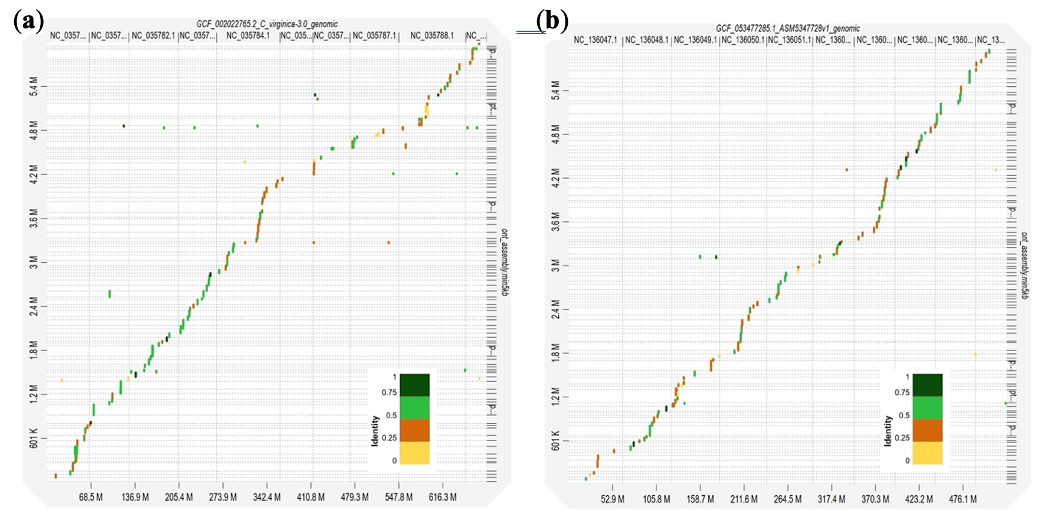
\includegraphics[width=1\linewidth]{manuscript/working-template/alignment.png}
    \caption{Comparison between de novo assembly from ULDNA Nanopore sequences and two reference genomes showing the 10 chromosomes of \textit{Crassostrea virginica} (a) Gómez-Chiarri et al. 2015 reference and (b) Hoh et al. 2025 reference.}
    \label{fig:alignment}
\end{figure}

\begin{figure}
    \centering
    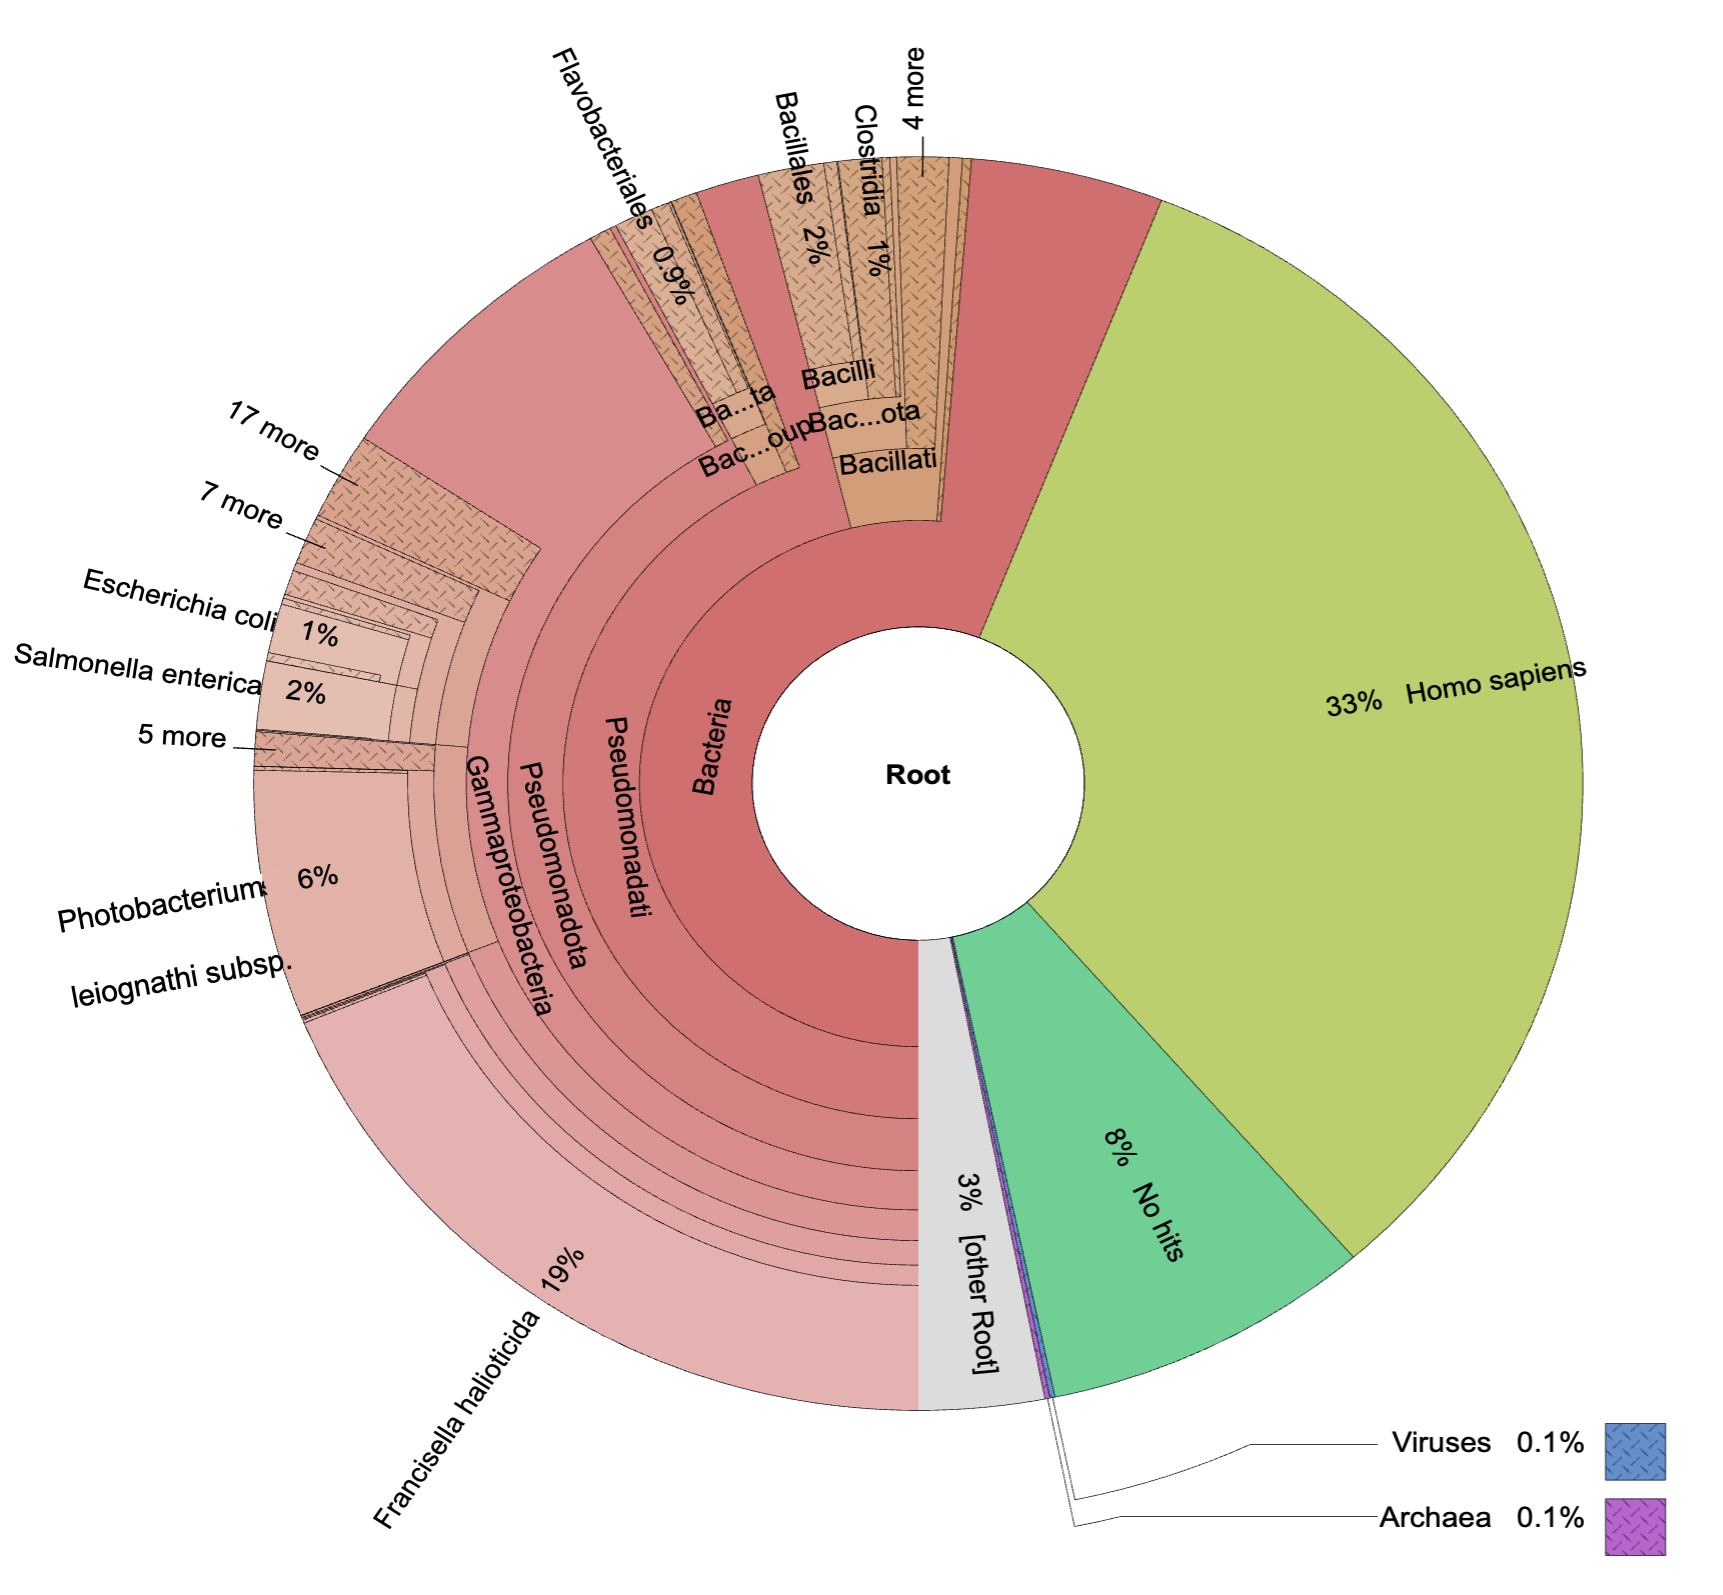
\includegraphics[width=0.8\linewidth]{manuscript/working-template/krona.png}
    \caption{Unmapped reads (5.4\%) from ULDNA Nanopore sequences. Krona output of unmapped reads from ULDNA sequencing of \textit{C. virginica} haemocytes. Reads are shown to the species level where possible.}
    \label{fig:krona}
\end{figure}

\begin{table}[ht]
\caption{Top 10 taxonomic classes represented in unmapped reads generated from \textit{C. virginica} haemocyte ULDNA sequencing.}
\label{table:taxonomy}
\begin{tabular}{@{}lrr@{}}
\toprule
Class & No. of reads & \% of all unmapped reads \\
\midrule
Gammaproteobacteria & 8892 & 41.79 \\
Mammalia & 6952 & 32.67 \\
Bacilli & 413 & 1.94 \\
Clostridia & 225 & 1.06 \\
Flavobacteriia & 202 & 0.95 \\
Actinomycetes & 167 & 0.78 \\
Alphaproteobacteria & 82 & 0.39 \\
Spirochaetia & 58 & 0.27 \\
Epsilonproteobacteria & 49 & 0.23 \\
Cyanophyceae & 44 & 0.21 \\
\botrule
\end{tabular}
\end{table}

\section{Discussion}
At the time of this study, there were no mollusk-specific published reports that documented successful ULDNA extraction from mollusks with downstream demonstration of ultra-long reads or a mollusk genome assembly from UHMW DNA. The study of \cite{dotto-maurel_evaluation_2025} found traditional HMW DNA extraction kits were suitable for successful extraction of OSHV1 (a herpes virus of ostreid oysters), but our attempts to obtain eastern oyster ULDNA using each of the recommended kits yielded no ULDNA. Modification \cite{brown_population_1989} provided quantities of high molecular weight DNA that appeared to be sufficient for Nanopore library preparation and ULDNA sequencing. However, the read lengths obtained from the oyster ULDNA preparation (N50 16kb) were shorter than the expected N50 length (50-100kb) and the number of ULDNA contigs obtained (105) fell considerably below the expected range from a PromethION flow cell of 2,500-4,500 contigs. Lower contig numbers most likely reflected that a portion of the fragments were considerably shorter than the optimal $>$ 50kb in length. This implies that pulsed-field gel electrophoresis (PFGE) would be more appropriate for the DNA integrity checking step and if necessary, the highest molecular weight DNA would be excised and extracted from the gel. Alternatively, library preparation for this type of DNA may need to be further modified from the recommended protocol. Nevertheless, sufficient ULDNA was generated to successfully assemble 91.4\% of the \textit{C. virginica} genome.

Aside from the lower output than expected, some other aspects of this study produced unexpected results, which requires some explanation for discrepancies. Although the majority of generated reads successfully mapped to the eastern oyster reference genomes, de novo assembly proved challenging, with only 57.6\% of the de novo assembly matching the published eastern oyster reference genomes (Table \ref{table:output}, Figure \ref{fig:alignment}). A likely explanation for this discrepancy is the extensive genome-wide duplications and repetitive regions within the eastern oyster genome \cite{kamalay_dna_1976, modak_extensive_2021}. Repetitive regions in the eastern oyster genome are estimated to be about 35-54\% of the total genome. These repetitive regions prove challenging for \textit{de novo} genome assembly \cite{liao_current_2019}, which could account for the dissimilarity between the established reference genomes and the de novo one generated in this study. Additionally, in extensively repetitive regions, reads often are misassembled, leading to gaps in coverage \cite{treangen_repetitive_2012, wang_read_2019}. To address these concerns in future studies, alternative assemblies that address extensive repetitive regions should be considered in the pipeline, such as RepAHR \cite{liao_current_2019}.

Very minimal non-oyster DNA (~5\% of reads did not map to the eastern oyster reference genomes) was found within the ultra-long samples, demonstrating utility of haemocytes for this protocol. Oyster haemolymph has been shown to host a variety of bacteria, protists, and viruses \cite{dupont_oyster_2020}. When analyzing the unmapped reads to determine species classification, several interesting identifications became present. \textit{Francisella halioticida}, comprised 19\% of the non-oyster reads. This pathogen, causing macroscopic lesions in several bivalves species including blue mussels \cite{bouras_influence_2024, cano_first_2022}, scallops \cite{kawahara_parallel_2019, kawahara_four-year_2024}, and abalone \cite{brevik_francisella_2011, kamaishi_mass_2010}, has not been identified previously in oysters from Great Bay Estuary. \textit{Photobacterium leiognathi subsp. mandapamensis} is a gram-negative bacterium in the same family as \textit{Vibrio parahaemolyticus}, comprised 6\% of non-oyster reads. This pathogen is known to exist in Great Bay Estuary eastern oysters \cite{hartwick_forecasting_2019}. In addition to numerous bacteria found, \textit{Homo sapiens} DNA accounted for 33\% of unmapped reads. It has been well-documented that untreated or partially treated sewage makes its way into Lamprey River either from faulty septic systems or by direct discharge, feeding directly into GBE \cite{piscataqua_region_estuaries_partnership_state_2023}. Given that oysters have an open circulatory system and the location near the mouth Lamprey River where the oysters were sampled, it is reasonable to suspect that untreated wastewater could have contributed to the sewage-related bacterial and human reads that were identified in the unmapped read set.

\section{Conclusions}
Continued advancement of genomic techniques is becoming increasingly important for in-depth studies of both economically and environmentally important marine organisms, such as the eastern oyster. However, as -omics techniques continually advance, methodologies optimized for “difficult” marine organisms, such as mollusks, struggle to keep pace. This study resulted from the need to optimize ULDNA extraction methods from eastern oysters to use with the Oxford Nanopore Technologies ULNA sequencing kit. The results from this sequencing analysis show that although standard ultra-long estimations developed by ONT were not reached, many ultra-long reads were generated and used throughout downstream analyses. Combining ultra-long scaffolds with the existing eastern oyster reference genomes could provide telomere-to-telomere assembly of the eastern oyster genome. This would expose hard-to-reach areas, such as repetitive regions and heterochromatic regions, allowing for the expansion of future studies of the eastern oyster genome.

\bmhead{Acknowledgements}
Thanks are due to members of the Brown Ecological Genetics Lab for assistance with field tasks: Kelsey Meyer, Taja Sims-Harper, and Grant Milne, and various undergraduates. David Shay helped with vessels for sample collection. Ray Grizzle, Robert Atwood, Brianna Group, Kelley Thomas, and Elizabeth Harvey provided logistical and experimental design advice.

\section*{Declarations}
\bmhead{Author Contributions}
Conceptualization, A.S., M.J., and B.B.; methodology, A.S., K.A., M.J. and B.B.; software, A.S.; formal analysis, A.S. and B-Y.L.; investigation, A.S., C.G., and K.A.; resources, B.B.; data curation, A.S. and B-Y. L.; writing—original draft preparation, A.S.; writing—review and editing, B.B., B-Y.L. C.G., K.A. and M.J.; visualization, A.S. and B-Y.L.; supervision, B.B.; project administration, B.B.; funding acquisition, B.B. All authors have read and agreed to the published version of the manuscript.
\bmhead{Funding}
Partial funding for this research was provided by the New Hampshire Agricultural Experiment Station [scientific contribution number TBD], supported by the USDA National Institute of Food and Agriculture Hatch Project Numbers 7004018 and 7005577 and the state of New Hampshire awarded to B.B.. Partial funding also was provided by Richmond-Durham Enterprises, LLC to B.B.. Partial funding also was provided via a New Hampshire Sea Grant Graduate Fellowship awarded to A.S.
\bmhead{Data Availability}
Sequence data for mapped and unmapped reads were accessed to NCBI TBD. 
\bmhead{Code Availability}
Analyses can be found at https://github.com/astrickland4/oyster-uldna.
\bmhead{Conflicts of Interest}
The authors declare no conflicts of interest.

\bibliography{oyster-uldna}


\end{document}
